\documentclass{article}

\usepackage[a4paper, left=1.5cm, right=1.5cm, top=1.0cm, bottom=1.0cm]{geometry}
\usepackage{graphicx} 
\usepackage{polski}
\usepackage[utf8]{inputenc}
\usepackage{setspace} % \onehalfspacing
\usepackage{lipsum}
\usepackage{array, xcolor}

\newcolumntype{C}[1]{>{\centering\arraybackslash}m{#1}}
\newcolumntype{R}[1]{>{\raggedleft\arraybackslash}m{#1}}

\onehalfspacing
\hyphenpenalty=5000
\tolerance=1000

\newcommand{\header}[1] 
{
	\textbf{\large #1}
	\vspace{0.005\textheight}
	\hrule 
	\vspace{0.005\textheight}
}

\pagenumbering{gobble} 
\begin{document}  
\noindent
\LARGE 
\centering
CURRICULUM VITAE \\
\large
\begin{tabular}{@{}p{0.70\textwidth} r}
	 \begin{minipage}{0.70\textwidth}
		\begin{tabular}{@{}l l} 
		\textbf{Name}: 		& 	Bartłomiej Kordek\\
		\textbf{Date and place of birth}: & 1989.08.02 Nowy Dwór Mazowiecki \\
		\textbf{Address}:		&	ul. Szczęśliwicka 8/135, 02-352 Warszawa\\
		\textbf{Telephone}:	& 507-832-154\\
		\textbf{E-mail}:	&	 bartekordek@gmail.com\\
		\end{tabular}	
	\end{minipage}
	
	& 
	\begin{minipage}{0.30\textwidth} 
		\begin{center}
			{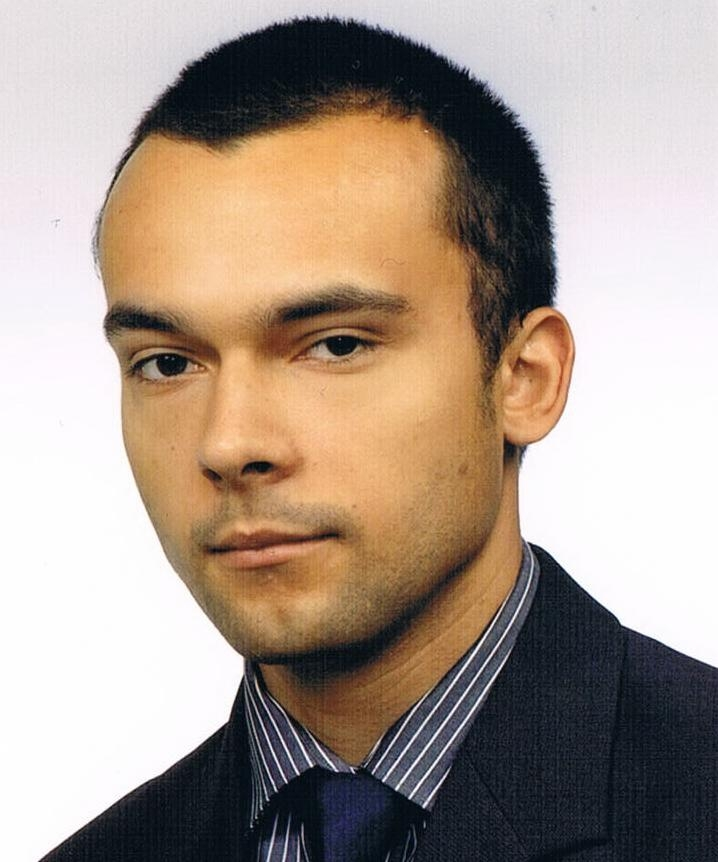
\includegraphics[width=0.70\textwidth]{./Picture}}
		\end{center} 
	\end{minipage}
\end{tabular}
\flushleft

\large
\header{Education}
\begin{tabular}{@{} m{0.60\textwidth} R{0.37\textwidth} }
\textbf{Warsaw University of Technology}	& {2008 - 2012} \\
\end{tabular}
 B.S. in Technical Physics, Specialisation: Materials \& Nanostructures.\\
Thesis title: ”Experimental analysis of correlation between temperature of glass transition and thermal linear  expansion coefficient in chosen amorphous metallic alloys.”
\begin{tabular}{@{} m{0.60\textwidth} R{0.37\textwidth} }
\textbf{School of Computer Science and Managment WIT}	& {2013 - today} \\
\end{tabular}
External studies - Computer Science.
\flushleft

\header{Experience}

\begin{tabular}{@{} m{0.60\textwidth} R{0.37\textwidth} }
\textbf{Nitreal Games}	& {2015-11 - Today} 
\end{tabular}
Software Developer\\
\begin{itemize}
	\item Improvement and maintenance of (3-D) analysis software (\texttt{C++}).
	\item Improvement and maintenance of (3-D) scenario editor (\texttt{C\#} \ \texttt{C++}).
	\item Improvement and maintenance of (2.5D) game (\texttt{Javascript}).
\end{itemize}

\begin{tabular}{@{} m{0.60\textwidth} R{0.37\textwidth} }
\textbf{Accenture Polska}	& {2015-06 - 2015-10} 
\end{tabular}
Junior Trainee\\
\begin{itemize}
	\item Creation of various types of automatizations (\texttt{VBA}, \texttt{Blue Prism}, \texttt{C\#}, \texttt{Selenium}).
	\item Creation of documentation (including High Level Design).
	\item Optimization of processes. 
\end{itemize}

\begin{tabular}{@{} m{0.60\textwidth} R{0.37\textwidth} }
\textbf{Samsung Electronics Polska}	& {2015-01 - 2015-03} 
\end{tabular}
Junior Software Developer\\
\begin{itemize}
	\item Management and improvement of automated test environment.
	\item Software development in \texttt{C/C++}, \texttt{Python} and \texttt{BASH} shell.
	\item Management and improvement of continuous integration environment.
	\item Bug fixing.
	\item Preparation of documentation (\LaTeX).
\end{itemize}

\begin{tabular}{@{} m{0.60\textwidth} R{0.37\textwidth} }
	\textbf{Samsung Electronics Polska}	& {2014-08 - 2014-12} 
\end{tabular}
Trainee\\
\begin{itemize}
	\item Management and improvement of continuous integration environment.
	\item Software development (\texttt{BASH} shell, \texttt{C\#}, \texttt{C/C++} and \texttt{Python}).
	\item Preparation of documentation (\LaTeX). 
\end{itemize}

\begin{tabular}{@{} m{0.60\textwidth} R{0.37\textwidth} }
\textbf{Office worker in commune office} & {2013.03 - 2014-06} 
\end{tabular}
\begin{itemize}
	\item Making, editing and management of various types of documents.
	\item Creation and maintenance of website.
	\item Reception of enquirers.
	\item Maintenance of various electronic equipment such as computers and printers.
\end{itemize}

\begin{tabular}{@{} m{0.60\textwidth} R{0.37\textwidth} }
\textbf{Institute of Electron Technology PAN} & {2011.07} 
\end{tabular}
Trainee:
\begin{itemize}
	\item Writing laser power control software (\texttt{Labview}).
	\item Creating a Bragg mirror for a fixed wavelength.
	\item Writing software various for servomechanisms (\texttt{Labview}).
\end{itemize}

\textbf{\large Skills}
\vspace{0.005\textheight}
\hrule 

\begin{itemize}
	\item Object Oriented Programming.
	\item boost library.
	\item Clean code techniques.
	\item Experience in using \LaTeX \hspace {0.01\textwidth}typesetting system.
	\item Operating systems: \texttt{Linux} and \texttt{Windows}.
	\item Languages: \texttt{BASH} shell, \texttt{C}, \texttt{C++}, \texttt{C\#}, \texttt{Java}, \texttt{Labview\texttt}, \texttt{Python} and \texttt{R}.
	\item Experience in programming \texttt{AVR} microcontrollers.
	\item \texttt{Mathematica} computation system and \texttt{ROOT} data analysis framework.
	\item Development environments: \texttt{Eclipse}, \texttt{VIM} and \texttt{Visual Studio}.
	\item GIT and Perforce revision control systems.
	\item Experience in creating websites (\texttt{HTML} and \texttt{CSS}).
	\item Basic knowledge of electronics and electrotechnics.
	\item \texttt{JIRA} and \texttt{FishEye}.
\end{itemize}

\header{Additional information}
Driving license - B category.\\
English language - passed B2 level exam.\\
Experience in using various laboratory equipment such as multimeters, oscilloscopes, power supplies and generators.\\
\header{Interests and activities}
Music, guitars, electronics, programming, DIY, astronomy, physics, books, movies and sports.
\vspace{0.05\textheight}
\noindent\newline
\scriptsize
\begin{minipage}{\textwidth}
	I hereby declare that all the facts and information provided for this cover letter and CV are true. I allow my personal data stated in the abovementioned applications to be processed for the purpose of recruitment, in accordance with the Personal Data Protection Act dated 29/08/1997 (Dz.Ust.No.133, item 883).
\end{minipage}

\end{document}
